\documentclass[11pt]{beamer}
\usepackage[utf8]{inputenc}
\usepackage{graphicx, epsfig}
\usepackage{amsmath,mathrsfs,amsfonts,amssymb}
%\usepackage{subfig}
\usepackage{floatflt}
\usepackage{epic,ecltree}
\usepackage{mathtext}
\usepackage{fancybox}
\usepackage{fancyhdr}
\usepackage{multirow}
\usepackage{enumerate}
\usepackage{epstopdf}
\usepackage{multicol}
\usepackage{algorithm}
\usepackage[noend]{algorithmic}
\usepackage{tikz}
\usepackage{blindtext}
\usetheme{default}%{default}%{Singapore}%{Warsaw}%{Warsaw}%{Darmstadt}
\usecolortheme{default}
\setbeamerfont{title}{size=\Huge}
\setbeamertemplate{footline}[page number]{}


\makeatletter
\newcommand\HUGE{\@setfontsize\Huge{35}{40}}
\makeatother    

\setbeamerfont{title}{size=\HUGE}
\beamertemplatenavigationsymbolsempty

% latin bold lower
\newcommand{\ba}{\mathbf{a}} 
\newcommand{\bc}{\mathbf{c}} 
\newcommand{\be}{\mathbf{e}} 
\newcommand{\bh}{\mathbf{h}} 
\newcommand{\bp}{\mathbf{p}} 
\newcommand{\bt}{\mathbf{t}} 
\newcommand{\bs}{\mathbf{s}} 
\newcommand{\bu}{\mathbf{u}} 
\newcommand{\bv}{\mathbf{v}} 
\newcommand{\bw}{\mathbf{w}} 
\newcommand{\bx}{\mathbf{x}} 
\newcommand{\by}{\mathbf{y}} 
\newcommand{\bz}{\mathbf{z}} 

% latin bold upper
\newcommand{\bA}{\mathbf{A}} 
\newcommand{\bB}{\mathbf{B}} 
\newcommand{\bC}{\mathbf{C}} 
\newcommand{\bI}{\mathbf{I}} 
\newcommand{\bL}{\mathbf{L}} 
\newcommand{\bM}{\mathbf{M}} 
\newcommand{\bQ}{\mathbf{Q}} 
\newcommand{\bT}{\mathbf{T}} 
\newcommand{\bU}{\mathbf{U}} 
\newcommand{\bV}{\mathbf{V}} 
\newcommand{\bW}{\mathbf{W}} 
\newcommand{\bX}{\mathbf{X}} 
\newcommand{\bY}{\mathbf{Y}} 
\newcommand{\bZ}{\mathbf{Z}} 

% latin cal upper
\newcommand{\cG}{\mathcal{G}} 
\newcommand{\cL}{\mathcal{L}} 
\newcommand{\cN}{\mathcal{N}} 
\newcommand{\cS}{\mathcal{S}} 
\newcommand{\cT}{\mathcal{T}} 
\newcommand{\cW}{\mathcal{W}} 
\newcommand{\cX}{\mathcal{X}} 
\newcommand{\cZ}{\mathcal{Z}} 

% latin bb upper
\newcommand{\bbE}{\mathbb{E}} 
\newcommand{\bbI}{\mathbb{I}} 
\newcommand{\bbP}{\mathbb{P}} 
\newcommand{\bbR}{\mathbb{R}} 

% greek bold lower
\newcommand{\bepsilon}{\boldsymbol{\epsilon}} 
\newcommand{\btheta}{\boldsymbol{\theta}} 
\newcommand{\blambda}{\boldsymbol{\lambda}} 
\newcommand{\bpi}{\boldsymbol{\pi}} 
\newcommand{\bmu}{\boldsymbol{\mu}} 
\newcommand{\bsigma}{\boldsymbol{\sigma}} 
\newcommand{\bphi}{\boldsymbol{\phi}} 

% greek bold upper
\newcommand{\bSigma}{\boldsymbol{\Sigma}} 

\DeclareMathOperator*{\argmin}{arg\,min}
\DeclareMathOperator*{\argmax}{arg\,max}
\newcommand{\createdgmtitle}[1]{\title[\hbox to 56mm{Mathematical Forecasting Methods \hfill\insertframenumber\,/\,\inserttotalframenumber}]
	{\vspace{1.5\cm} \\ Mathematical Forecasting Methods \\ {\Huge Лекция #1}}
	\author{}
	\institute{
	МФТИ
	} 
	\date{Осень, 2023}
}

\newcommand\myfootnote[1]{%
  \tikz[remember picture,overlay]
  \draw (current page.south west) +(1in + \oddsidemargin,0.5em)
  node[anchor=south west,inner sep=0pt]{\parbox{\textwidth}{%
      \rlap{\rule{10em}{0.4pt}}\raggedright\scriptsize \textit{#1}}};}

\newcommand\myfootnotewithlink[2]{%
  \tikz[remember picture,overlay]
  \draw (current page.south west) +(1in + \oddsidemargin,0.5em)
  node[anchor=south west,inner sep=0pt]{\parbox{\textwidth}{%
      \rlap{\rule{10em}{0.4pt}}\raggedright\scriptsize\href{#1}{\textit{#2}}}};}
\createdgmtitle{4}
\usepackage{tikz}
\usepackage{amsmath}
\usepackage[english,russian]{babel}
\usepackage[labelformat=empty]{caption}

\usetikzlibrary{arrows,shapes,positioning,shadows,trees}
\newcommand*{\defeq}{\stackrel{\text{def}}{=}}

%--------------------------------------------------------------------------------
\begin{document}
%--------------------------------------------------------------------------------
\begin{frame}[plain]
%\thispagestyle{empty}
\titlepage
\end{frame}
%======
\begin{frame}{Краткое повторение}
\textbf{Модель SARIMAX($p, q, d; P, Q, D$)} приводит временной ряд к стационарному виду и прогнозирует с наперед заданной точностью (по Теореме Вольда).
\begin{equation*}
    \begin{aligned}
    x_t = \mu &
    + \underbrace{\phi_1 x_{t-1} + \phi_2 x_{t-2} + ...}_{p\text{ слагаемых AR}}
    + \underbrace{u_t + \theta_1 u_{t-1} + \theta_2 u_{t-2} + ...}_{q\text{ слагаемых MA}}\\
    &+ \underbrace{\alpha_1 x_{t-S} + \alpha_2 x_{t-2S}+ ...}_{P\text{ сезонных слагаемых AR}}
    + \underbrace{\eta_1 u_{t-S} + \eta_2 u_{t-2S}+ ...}_{Q\text{ сезонных слагаемых MA}}\\
    &+ \underbrace{\beta_1 z_1 + \beta_2 z_2 + \beta_3 z_3+ ...}_{\text{внешние переменные, не звисящие от } x_t},
    \end{aligned}
\end{equation*}
где $\phi, \theta, \alpha, \eta, \beta$ --- настраивамемые параметры модели,\\
$x_t$ --- значения временного ряда (продифференцированные d и D сезонных раз),\\
$u_t$ --- значения шумов,\\
$z_i$ --- внешние (экзогенные) перменные.
\end{frame}
%=======
\begin{frame}{Краткое повторение}
\begin{itemize}
\item Если ранее полагалось, что $u_t \sim WN(0,1)$, то теперь возмущения будут моделироваться с меняющейся во времени дисперсией $\sigma_t^2$: $$u_t =  z_t \sqrt{\sigma_t^2},$$ где $z_t \sim WN(0,1)$.
\item  Моделирвоание дисперсии как процесс AR(q), используя квадраты оцененных остатков.
\item \textbf{ARCH}($p$): $ \sigma_t^2 = \alpha_0 + \alpha_1 u_{t-1}^2 + \alpha_2 u_{t-2}^2 + \dots + \alpha_p u_{t-p}^2$.
\item Обобщение модели с предположением, что дисперсия зависит от своих прошлых значений.\\
\item\textbf{GARCH}($p, q$):
$$ \sigma_t^2 = \omega + \sum_{i=1}^p \alpha_i u_{t-i}^2 + \sum_{j=1}^q \beta_j \sigma_{t-j}^2$$
Здесь $\omega > 0, \ \alpha_i \geq 0 \ \forall i = \overline{1, p}, \ \beta_j \geq 0 \ \forall j = \overline{1, q}$.
\end{itemize}
\end{frame}
%=======
\begin{frame}{Введение в нейронные сети для временных рядов}
    \item Задача прогнозирования временного ряда $x_{t} \approx f_{t,N}(x_{t-1},...x_{t-N};w) =: \hat{x}_{t}$
\end{frame}
% %=======



\begin{frame}{Механизм Attention и модель Transformer}

\begin{figure}
    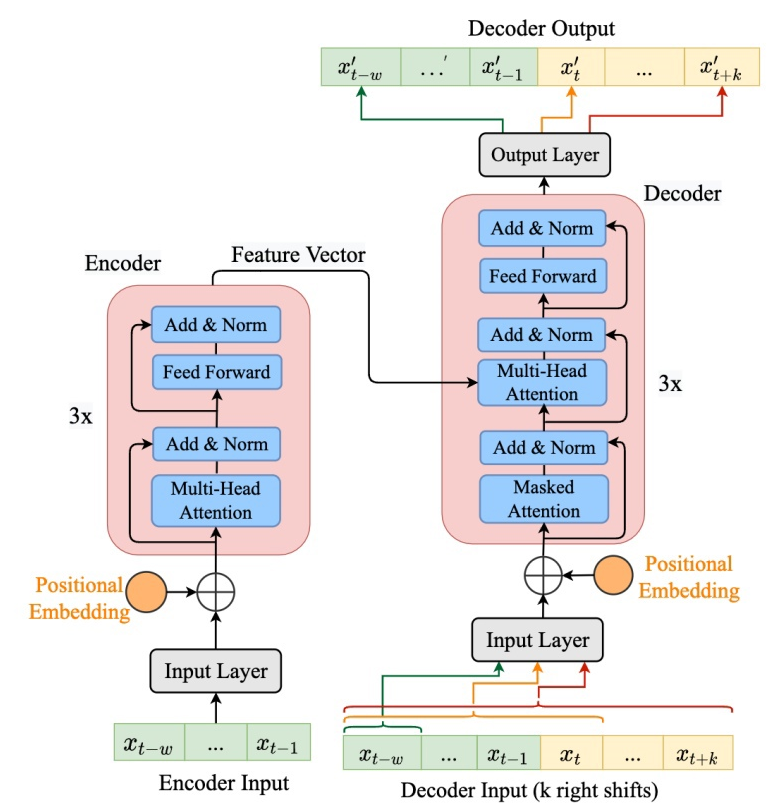
\includegraphics[width=0.7\linewidth]{lecture_4/figs/Transformer.png}
\end{figure}
\end{frame}
%=======

\begin{frame}{Резюме}
\begin{itemize}
    \item Линейные модели сильно органичены.
    \item Нейронные сети моделируют нелинейные зависимости.
    \item Модели сверточных нейронных сетей CNN применяются к предыстории и позволяют извлекать сложные закономерности.
    \item Рекуррентные нейронные сети RNN хранят внутреннее состояние и эффективнее работают с последовательностями.
    \item Модификации классической RNN (например, LSTM и GRU) лучше справляются с затуханием и взрывом градиента.
\end{itemize}
\end{frame}
\end{document} 